\documentclass[10]{article}
\usepackage[margin=1in]{geometry}

\usepackage{graphicx}
\graphicspath{{../../data/features/visualize/}}
\usepackage{fancyvrb,color,amssymb,float,alltt,verbatim}
\usepackage{amsmath,mathtools,listings,multicol,hyperref,enumerate}
\usepackage[usenames,dvipsnames,svgnames,table,hyperref]{xcolor}

\usepackage[style=chem-acs]{biblatex}
\bibliography{milestone}

\usepackage{color}

\begin{document}
\begin{center}
\huge{\textbf{CS229 - Milestone Report}} \\
\end{center}
\begin{center}
\normalsize{11 13 2015} \\

Keri A. McKiernan \\
Joe Napoli
\end{center}
%------------------------------------------------------------------------------%
\section*{DW-NOMINATE for candidate selection}
Public interest has become increasingly concentrated on the effect of money in politics. Specifically, the Citizens United v. FEC Supreme Court ruling maintained the legality of unrestricted political expenditures by corporate and union entities. As a result, there has been a proliferation of super PAC, or `political action committee',  organizations. While these organizations are not permitted to make contributions directly to candidates’ campaigns, they may engage in unlimited independent spending and there is no restriction on the amount of funds they can accept from donors. These legal developments beg the question: Can one predict explicitly the influence of donors over politicians to whom they give? \\

The research of Poole and Rosenthal has focused on quantifying the political ideology of politicians [cite]. In particular, they actively develop methods for calculating "ideal points" for candidates. The DW-NOMINATE method calculates a legislator’s overall probability of voting "yea" on an item of legislation as the sum of a deterministic utility value and a random error [cite]. "Ideal point" coordinates were obtained for legislators by maximizing the log likelihood function

\[ \sum_{t=1}^{T} \sum_{i=1}^{p_t} \sum_{j=1}^{q_t} \sum_{\tau = 1}^{2} C_{ij \tau t} \ln P_{ij \tau t} \]

\noindent where $P_{ij \tau t}$ is the probability of voting for choice $\tau$ (yes or no) and $C_{ij \tau t} = 1$ if that probability accurately predicts the vote [cite]. Indexes $j$, $i$, and $t$ sum over roll call votes, legislators, and legislative sessions, respectively. Ideal points are constrained to lie within the interval $\left[ -1,1 \right]$ and are two-dimensional quantities. A common interpretation of the first coordinate is that it reflects the divide between the Republican and Democratic parties, whereas the second coordinate is more highly correlated with intra-party division [cite]. While a full congressional voting record is not available for candidates who are new to office, campaign finance data is readily available. It would be useful to be able to predict the ideal point of a candidate even before they have established a congressional voting record. Furthermore, the ability to do so would help elucidate a relationship between monetary contributions to candidates and the voting patterns those contributions may effect.\\

We have collated freely available campaign finance [cite] and DW-NOMINATE ideal point [cite] datasets and performed a principal component analysis on the feature set extracted therefrom. The original scope of our project has been narrowed due to a reduction in the size of our group. While originally we had planned to investigate anomalous voting behavior and the ability to predict it solely by examining campaign finance data, we have shifted our focus on training a model to predict DW-NOMINATE ideal points, which directly reflect ideological stances and inter-/intra-party divisions [cite]. This shift has been prompted by datasets that were relatively more sparse than expected as well as the challenge of collating them.\\

\section*{Feature determination}

\begin{figure}[H]
\section*{PCA of features}
\centering
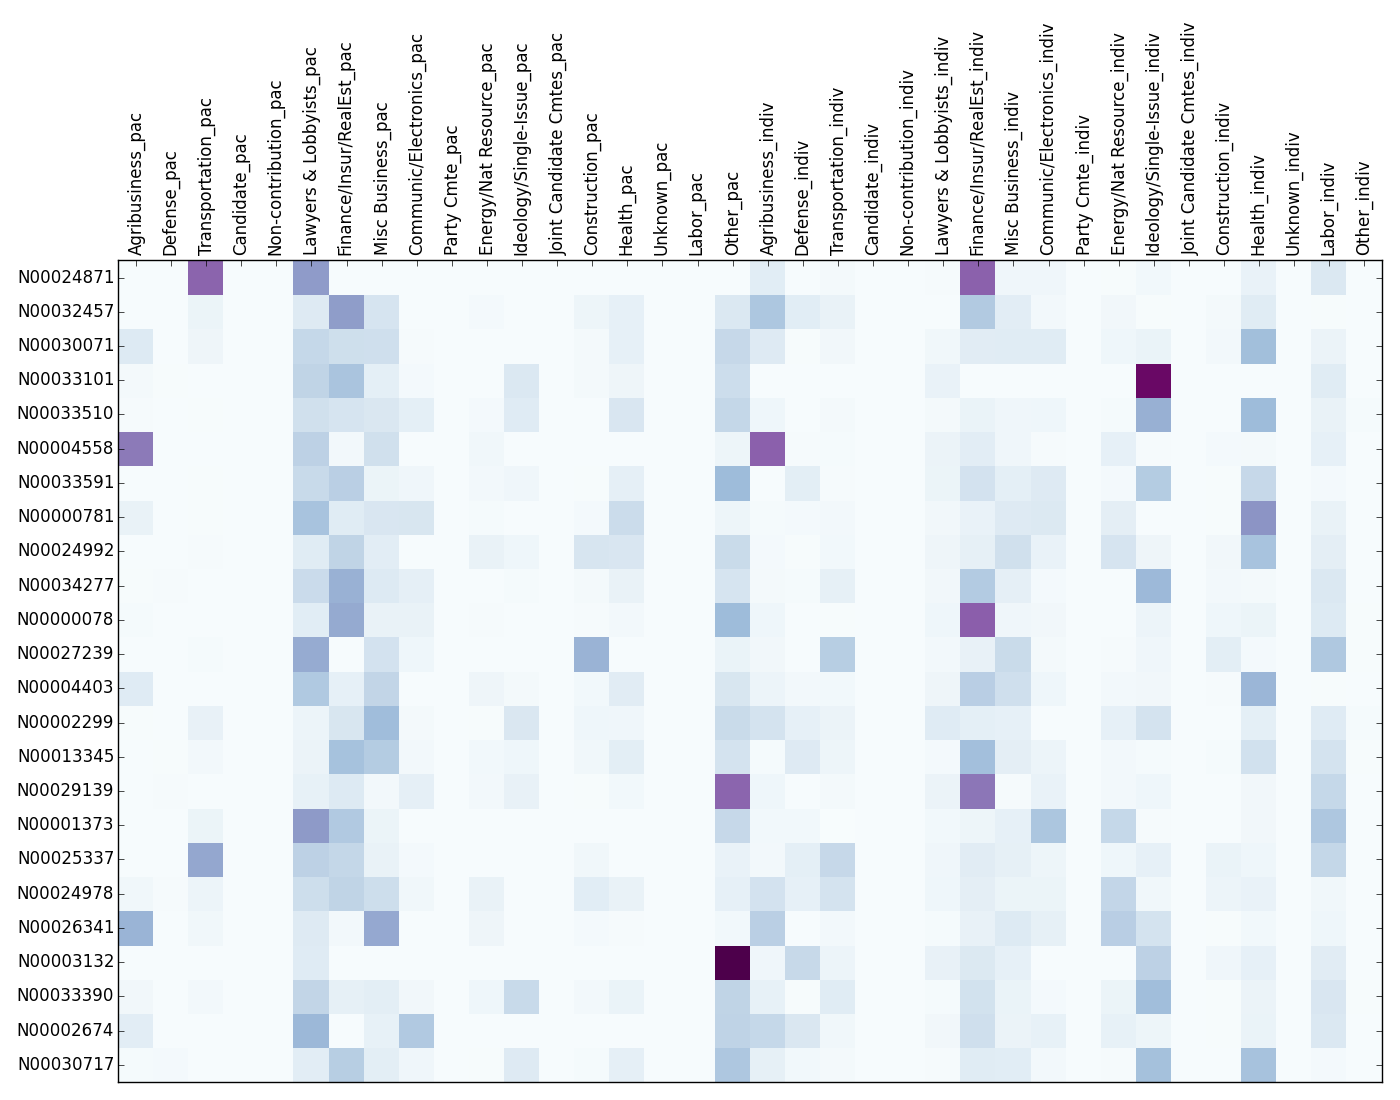
\includegraphics[width=.9\textwidth]{../../data/features/visualize/mod_2014_fm.png}
\caption{\label{fig:fmtrx}Heatmap of feature matrix.}
\end{figure}

\begin{figure}[H]
\centering
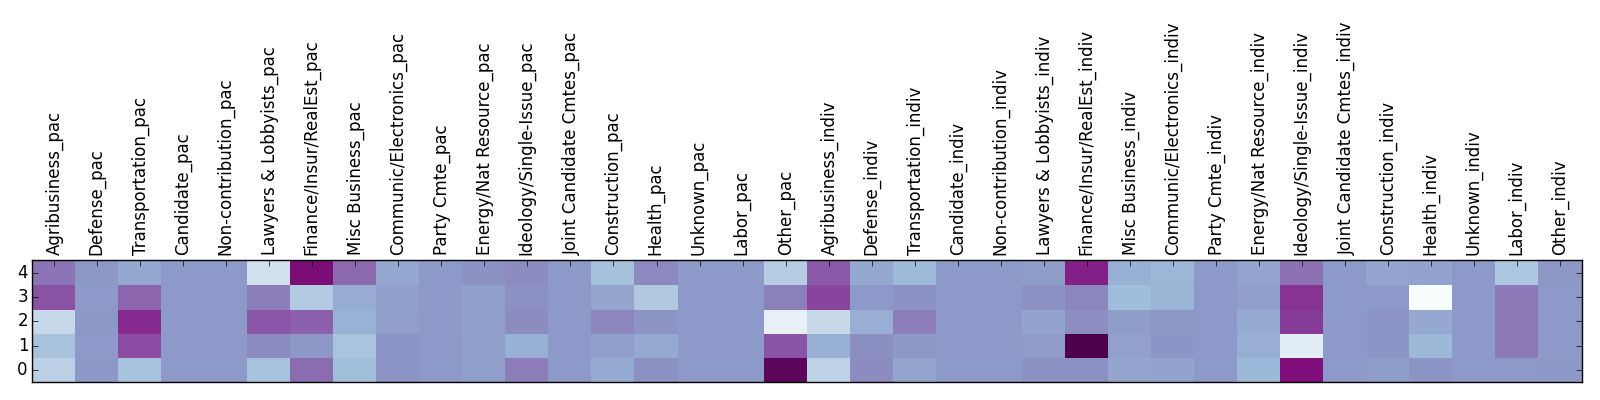
\includegraphics[width=.9\textwidth]{../../data/features/visualize/pcs.png}
\caption{\label{fig:fmtrx}Heapmap of PCA eigenvectors of feature matrix.}
\end{figure}

\end{document}
